\documentclass{article}
\usepackage{geometry}
\usepackage{amsmath}
\usepackage{amsfonts}
\usepackage{graphicx}
\usepackage{caption}
\usepackage{subcaption}
\usepackage{listings}
\usepackage{color}
\usepackage{hyperref}
\usepackage{tikz}
\usepackage{setspace}
\usepackage{booktabs}
\usepackage{siunitx}
\usetikzlibrary{3d}
\usepackage{pgfplots}
\pgfplotsset{compat=1.18}
\geometry{a4paper, margin=1in}
\doublespacing
\begin{document}

\begin{titlepage}
    \centering
    \vspace*{2cm} % Add vertical space at the top
    
    {\Huge \textbf{Homework 4}} \\
    
    \vspace{2cm}
    
    {\Large \textbf{Danen M. Pruitt}} \\
    
    \vspace{1.5cm}
    
    ENS, AFIT \\
    OPER 646: Reinforcement Learning \\
    May 2026
    
    \vfill % Pushes the following text to the bottom
    
\end{titlepage}

\newpage
\tableofcontents
\newpage

\section{Introduction}
In this assignment we will be considering the Gymnasium environment \textit{MountainCar-v0} and solving the agent's sequential decision problem using SARSA, Q-learning, and n-step SARSA. Across all of the algorithm implementations we configured them with the following stepsize TD learning rates.
\begin{align*}
    \alpha_n &= \alpha_a\left(\frac{1}{(n+1)^{\alpha_b}}\right)\\
    \epsilon_n &= \epsilon_a\left(\frac{1}{(n+1)^{\epsilon_b}}\right)
\end{align*}
We utilized a Latin hypercube design to tune the hyperparameters $\alpha_a, \alpha_b, \epsilon_a,\epsilon_b, \text{and } \mathcal{Q}^{init}$. Each was tuned with 60 design runs at 10 replications with 1000 episodes per replication. In each of the sections below, tables and figures will be presented. For brevity we will only look at the OLS and ANOVA results for each hyperparameter individually. Interaction terms can be found in the appendix.

\section{SARSA}
\begin{table*}[htbp]
\centering
\caption{Top 10 Results for SARSA\_onpolicy}
\label{tab:sarsa_results}
\resizebox{\textwidth}{!}{%
\begin{tabular}{rccccccccccccc}
\toprule
\textbf{Run Index} & $\alpha_a$ & $\alpha_b$ & $\epsilon_a$ & $\epsilon_b$ & \textbf{qinit} & \textbf{Sup EETDR} & \textbf{Sup EETDR hw} & \textbf{Mean Max EETDR} & \textbf{Mean Max EETDR ME} & \textbf{Time-Avg EETDR} & \textbf{Time-Avg EETDR ME} & \textbf{Secs per run} & \textbf{Alg Score} \\ \midrule
15 & 0.242 & 0.125 & 0.375 & 0.358 & 0.142 & -120.150 & 6.392 & -123.840 & 5.794 & -168.541 & 4.702 & 233.409 & -147.078 \\
14 & 0.592 & 0.175 & 0.358 & 0.275 & 0.942 & -114.700 & 7.026 & -121.720 & 6.493 & -173.997 & 4.241 & 239.248 & -148.223 \\
11 & 0.558 & 0.342 & 0.858 & 0.308 & 0.308 & -120.900 & 6.641 & -126.610 & 7.050 & -172.213 & 3.284 & 237.256 & -150.395 \\
41 & 0.992 & 0.358 & 0.175 & 0.325 & 0.542 & -125.950 & 6.997 & -131.360 & 8.752 & -161.449 & 4.939 & 222.038 & -150.622 \\
43 & 0.825 & 0.508 & 0.042 & 0.758 & 0.492 & -130.300 & 13.073 & -128.260 & 6.270 & -172.981 & 4.664 & 233.549 & -151.776 \\
6 & 0.275 & 0.108 & 0.742 & 0.425 & 0.175 & -127.650 & 5.670 & -126.750 & 7.231 & -174.418 & 4.187 & 241.776 & -151.831 \\
39 & 0.842 & 0.542 & 0.625 & 0.908 & 0.225 & -115.050 & 6.835 & -125.830 & 7.910 & -177.920 & 4.742 & 238.083 & -153.309 \\
21 & 0.342 & 0.142 & 0.125 & 0.825 & 0.442 & -127.100 & 6.089 & -136.030 & 9.456 & -160.759 & 4.919 & 221.156 & -153.563 \\
50 & 0.092 & 0.008 & 0.008 & 0.342 & 0.325 & -127.800 & 5.331 & -129.960 & 7.608 & -171.060 & 8.509 & 233.948 & -154.368 \\
42 & 0.442 & 0.392 & 0.025 & 0.442 & 0.608 & -115.850 & 7.017 & -130.890 & 8.335 & -173.129 & 4.163 & 234.303 & -154.452 \\ \bottomrule
\end{tabular}%
}
\end{table*}
Above is a table of the top 10 design runs for the SARSA on-policy algorithm with respect to algorithm score with the best design run's superlative policy EETDR of -124.25. The design run also gave us the following learning curve.
\begin{figure}[h]
    \centering
    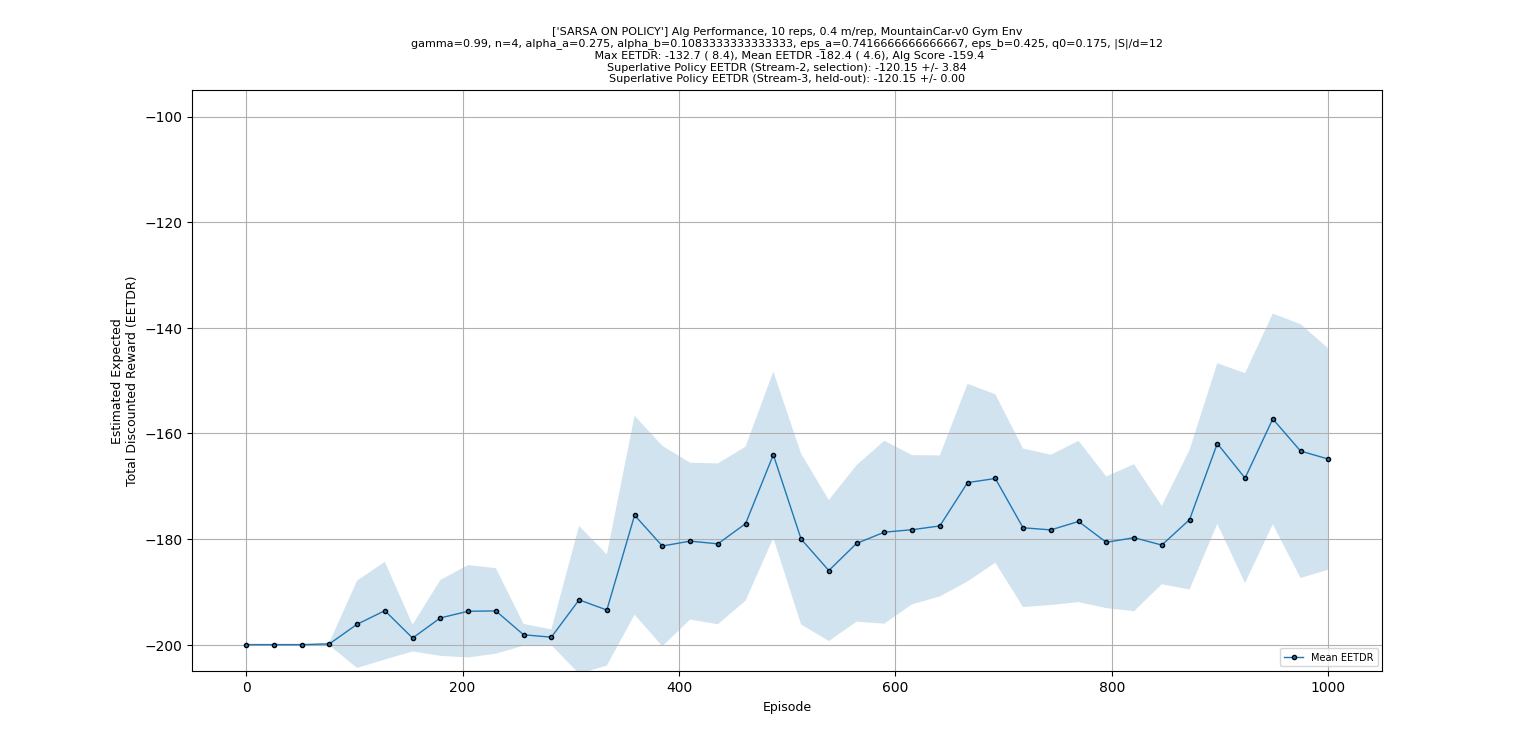
\includegraphics[width=0.8\textwidth]{SARSA LC.png}
    \caption{Learning Curve for Best SARSA run}
\end{figure}
\newpage
This figure illustrates the on-policy nature of the SARSA algorithm in the wide variance shaded regions. Since our epsilon values remain relatively large the on-policy algorithm explores more making the variance large. Below is a table of the OLS and ANOVA results for the SARSA algorithm.
\subsection*{OLS and ANOVA Regression Results}
\label{sec:statistical_results}

% Unified container for the tables
\begin{table}[htbp]
    \centering
    
    % --- FIRST ROW: OLS SUMMARY & OLS COEFFICIENTS SIDE-BY-SIDE ---
    \begin{subfigure}[b]{0.35\textwidth}
        \centering
        \caption{OLS Model Fit Summary}
        \label{tab:ols_summary}
        \begin{tabular}{lc}
            \toprule
            \textbf{Metric} & \textbf{Value} \\ 
            \midrule
            $R^2$ & 0.767 \\
            Adj. $R^2$ & 0.647 \\
            $F$-statistic & 6.415 \\
            Prob ($F$-stat) & $4.09 \times 10^{-07}$ \\
            Log-Likelihood & -217.290 \\
            AIC & 476.600 \\
            BIC & 520.600 \\ 
            \bottomrule
        \end{tabular}
    \end{subfigure}
    \hfill
    \begin{subfigure}[b]{0.58\textwidth}
        \centering
        \caption{ANOVA Type II Effects Table}
        \label{tab:anova_results}
        \begin{tabular}{lrrrc}
            \toprule
            \textbf{Variable} & \textbf{sum\_sq} & \textbf{df} & \textbf{$F$} & \textbf{PR($>F$)} \\ 
            \midrule
            $\alpha_a$ & 91.614 & 1.000 & 0.727 & 0.399 \\
            $\alpha_b$ & 104.986 & 1.000 & 0.834 & 0.367 \\
            $\epsilon_a$ & 86.722 & 1.000 & 0.689 & 0.412 \\
            $\epsilon_b$ & 1018.373 & 1.000 & 8.087 & 0.007 \\
            qinit & 67.197 & 1.000 & 0.534 & 0.469 \\ 
            \bottomrule
        \end{tabular}
    \end{subfigure}
    
    \vspace{5mm} % Vertical separation between OLS and ANOVA rows
    
    % --- SECOND ROW: ANOVA TABLE ---
    \begin{subfigure}[b]{0.9\textwidth}
    
        \centering
        \caption{OLS Coefficient Estimates}
        \label{tab:ols_coefficients}
        \begin{tabular}{lrrrcrc}
            \toprule
            \textbf{Variable} & \textbf{coef} & \textbf{std err} & \textbf{$t$} & \textbf{$P>|t|$} & \multicolumn{2}{c}{\textbf{[0.025 \quad 0.975]}} \\ 
            \midrule
            Intercept & -189.270 & 14.027 & -13.494 & 0.000 & -217.642 & -160.899 \\
            $\alpha_a$ & 28.662 & 33.604 & 0.853 & 0.399 & -39.310 & 96.633 \\
            $\alpha_b$ & -26.545 & 29.073 & -0.913 & 0.367 & -85.351 & 32.261 \\
            $\epsilon_a$ & 24.784 & 29.866 & 0.830 & 0.412 & -35.626 & 85.194 \\
            $\epsilon_b$ & 80.698 & 28.378 & 2.844 & 0.007 & 23.298 & 138.098 \\
            qinit & 23.925 & 32.753 & 0.730 & 0.469 & -42.324 & 90.174 \\ 
            \bottomrule
        \end{tabular}
    \end{subfigure}

\end{table}
From this table we see the only statistically significant variable is $\epsilon_b$. We are confident that it is the most significant as our model has high $R^2$ and Adj$R^2$ values telling us that it is a well fit and explanatory model. We shouldn't discount the other variables but it is not surprising that the algorithm, which is a TD algorithm, is more sensitive to the epsilon decay rate than learning rates or initial values. The higher our rate of decay the more we exploit rather than explore the policy we are currently following.  

\section{Q-Learning}
\begin{table*}[htbp]
\centering
\caption{Top 10 Results for Q\_learning\_offpolicy}
\label{tab:qlearning_results}
\resizebox{\textwidth}{!}{%
\begin{tabular}{rccccccccccccc}
\toprule
\textbf{Run Index} & $\alpha_a$ & $\alpha_b$ & $\epsilon_a$ & $\epsilon_b$ & \textbf{qinit} & \textbf{Sup EETDR} & \textbf{Sup EETDR hw} & \textbf{Mean Max EETDR} & \textbf{Mean Max EETDR ME} & \textbf{Time-Avg EETDR} & \textbf{Time-Avg EETDR ME} & \textbf{Secs per run} & \textbf{Alg Score} \\ \midrule
43 & 0.825 & 0.508 & 0.042 & 0.758 & 0.492 & -126.050 & 6.029 & -126.880 & 5.605 & -168.781 & 4.183 & 250.749 & -148.676 \\
15 & 0.242 & 0.125 & 0.375 & 0.358 & 0.142 & -127.950 & 6.586 & -123.900 & 4.504 & -174.079 & 5.080 & 263.673 & -148.706 \\
14 & 0.592 & 0.175 & 0.358 & 0.275 & 0.942 & -118.800 & 7.693 & -124.490 & 6.095 & -176.660 & 4.090 & 269.760 & -150.651 \\
53 & 0.692 & 0.525 & 0.575 & 0.875 & 0.458 & -118.600 & 6.044 & -126.100 & 6.346 & -174.841 & 3.157 & 258.703 & -150.667 \\
11 & 0.558 & 0.342 & 0.858 & 0.308 & 0.308 & -125.150 & 8.679 & -127.610 & 8.246 & -170.753 & 4.204 & 262.617 & -151.497 \\
41 & 0.992 & 0.358 & 0.175 & 0.325 & 0.542 & -127.550 & 5.287 & -137.330 & 4.676 & -160.762 & 5.582 & 242.912 & -151.742 \\
27 & 0.658 & 0.442 & 0.925 & 0.375 & 0.375 & -123.300 & 8.339 & -132.000 & 6.896 & -170.493 & 2.638 & 258.634 & -152.590 \\
36 & 0.192 & 0.242 & 0.225 & 0.608 & 0.192 & -119.400 & 8.021 & -130.350 & 7.251 & -171.768 & 3.982 & 256.396 & -152.861 \\
42 & 0.442 & 0.392 & 0.025 & 0.442 & 0.608 & -119.400 & 5.838 & -130.760 & 7.386 & -171.793 & 3.640 & 252.681 & -153.061 \\
32 & 0.075 & 0.042 & 0.308 & 0.175 & 0.475 & -118.950 & 7.355 & -129.340 & 6.707 & -175.987 & 2.930 & 266.639 & -153.195 \\ \bottomrule
\end{tabular}%
}
\end{table*}
Above is a table of the top 10 design runs for the Q-Learning off-policy algorithm with respect to algorithm score with the best design run's superlative policy EETDR of -126.05. The design run also gave us the following learning curve.
\newpage
\begin{figure}[h]
    \centering
    \includegraphics[width=0.8\textwidth]{Q_Learning LC.png}
    \caption{Learning Curve for Best Q-Learning run}
\end{figure}
Unlike the earlier SARSA algorithm, the Q-learning algorithm starts to learn the optimal policy earlier showing the power of the off-policy algorithm early on. The oscillations in the middle of the figure are likely due to the large exploration rate of $\epsilon_a$ forcing the agent to take more random actions rather than greedy ones but there is still steady improvement. Finally we notice that the variance shading is tighter due to the disconnect between the behavior policy and the target policy showing its ability to identify and maintain a high performing greedy policy even with the environmental noise. 
\newline
In the tables below we see that again the only statistically significant variable is $\epsilon_b$. It takes the highest coefficient value as well as the highest sum of squares value. Again, Q-learning is a TD learning algorithm so the rate at which we move from exploration to exploitation is extremely important to how well the algorithm performs and progresses in learning.
\newpage
\subsection*{OLS and ANOVA Regression Results}
\label{sec:q_learning_statistical_results}

% Unified container for the tables
\begin{table}[htbp]
    \centering
    
    % --- FIRST ROW: OLS SUMMARY & OLS COEFFICIENTS SIDE-BY-SIDE ---
    \begin{subfigure}[b]{0.4\textwidth}
        \centering
        \caption{Q-Learning Model Fit Summary}
        \label{tab:q_ols_summary}
        \begin{tabular}{lc}
            \toprule
            \textbf{Metric} & \textbf{Value} \\ 
            \midrule
            $R^2$ & 0.786 \\
            Adj. $R^2$ & 0.676 \\
            $F$-statistic & 7.168 \\
            Prob ($F$-stat) & $9.38 \times 10^{-08}$ \\
            Log-Likelihood & -214.630 \\
            AIC & 471.300 \\
            BIC & 515.200 \\ 
            \bottomrule
        \end{tabular}
    \end{subfigure}
    \hfill
    \begin{subfigure}[b]{0.58\textwidth}
        \centering
        \caption{Q-Learning ANOVA Type II Effects Table}
        \label{tab:q_anova_results}
        \begin{tabular}{lrrrc}
            \toprule
            \textbf{Variable} & \textbf{sum\_sq} & \textbf{df} & \textbf{$F$} & \textbf{PR($>F$)} \\ 
            \midrule
            $\alpha_a$ & 219.424 & 1.000 & 1.904 & 0.176 \\
            $\alpha_b$ & 44.162 & 1.000 & 0.383 & 0.540 \\
            $\epsilon_a$ & 74.924 & 1.000 & 0.650 & 0.425 \\
            $\epsilon_b$ & 1311.899 & 1.000 & 11.382 & 0.002 \\
            qinit & 107.902 & 1.000 & 0.936 & 0.339 \\ 
            \bottomrule
        \end{tabular}
    \end{subfigure}
    
    
    \vspace{5mm} % Vertical separation between OLS and ANOVA rows
    
    % --- SECOND ROW: ANOVA TABLE ---
    \begin{subfigure}[b]{0.9\textwidth}
        \centering
        \caption{Q-Learning Coefficient Estimates}
        \label{tab:q_ols_coefficients}
        \begin{tabular}{lrrrcrc}
            \toprule
            \textbf{Variable} & \textbf{coef} & \textbf{std err} & \textbf{$t$} & \textbf{$P>|t|$} & \multicolumn{2}{c}{\textbf{[0.025 \quad 0.975]}} \\ 
            \midrule
            Intercept & -196.515 & 13.419 & -14.645 & 0.000 & -223.657 & -169.372 \\
            $\alpha_a$ & 44.357 & 32.149 & 1.380 & 0.176 & -20.669 & 109.384 \\
            $\alpha_b$ & -17.216 & 27.814 & -0.619 & 0.540 & -73.475 & 39.042 \\
            $\epsilon_a$ & 23.036 & 28.572 & 0.806 & 0.425 & -34.756 & 80.829 \\
            $\epsilon_b$ & 91.592 & 27.149 & 3.374 & 0.002 & 36.679 & 146.506 \\
            qinit & 30.318 & 31.334 & 0.968 & 0.339 & -33.062 & 93.697 \\ 
            \bottomrule
        \end{tabular}
    \end{subfigure}

\end{table}

\section{n-step SARSA}
Below is a table of the top 10 design runs for the n-step SARSA algorithm with the additional column of n-steps. Here the best design run scored the highest of all three with a superlative policy EETDR of -115.45. The learning curve for this design run is also shown below.
\begin{table*}[htbp]
\centering
\caption{Top 10 Results for n\_step\_SARSA\_results.csv}
\label{tab:nstep_sarsa_results}
\resizebox{\textwidth}{!}{%
\begin{tabular}{rcccccccccccccc}
\toprule
\textbf{Run Index} & $\alpha_a$ & $\alpha_b$ & $\epsilon_a$ & $\epsilon_b$ & \textbf{qinit} & \textbf{n\_steps} & \textbf{Sup EETDR} & \textbf{Sup EETDR hw} & \textbf{Mean Max EETDR} & \textbf{Mean Max EETDR ME} & \textbf{Time-Avg EETDR} & \textbf{Time-Avg EETDR ME} & \textbf{Secs per run} & \textbf{Alg Score} \\ \midrule
11 & 0.558 & 0.342 & 0.858 & 0.308 & 0.308 & 5 & -115.450 & 0 & -122.730 & 7.453 & -145.831 & 5.649 & 200.855 & -127.732 \\
20 & 0.875 & 0.325 & 0.142 & 0.392 & 0.958 & 8 & -119.550 & 0 & -131.060 & 9.295 & -140.680 & 9.016 & 184.465 & -131.608 \\
41 & 0.992 & 0.358 & 0.175 & 0.325 & 0.542 & 3 & -118.100 & 0 & -130.990 & 8.047 & -147.120 & 5.349 & 187.639 & -131.848 \\
27 & 0.658 & 0.442 & 0.925 & 0.375 & 0.375 & 7 & -119.000 & 0 & -138.250 & 6.894 & -146.375 & 6.674 & 193.529 & -132.620 \\
1  & 0.425 & 0.625 & 0.458 & 0.625 & 0.158 & 9 & -116.350 & 0 & -139.030 & 12.529 & -151.154 & 7.306 & 194.182 & -133.194 \\
31 & 0.625 & 0.558 & 0.158 & 0.658 & 0.808 & 3 & -117.550 & 0 & -121.210 & 3.040 & -153.135 & 3.660 & 193.853 & -133.248 \\
15 & 0.242 & 0.125 & 0.375 & 0.358 & 0.142 & 6 & -118.550 & 0 & -137.990 & 7.958 & -150.900 & 4.874 & 198.906 & -133.440 \\
30 & 0.925 & 0.792 & 0.842 & 0.508 & 0.725 & 6 & -116.950 & 0 & -124.290 & 7.358 & -155.865 & 3.670 & 198.146 & -133.984 \\
6  & 0.275 & 0.108 & 0.742 & 0.425 & 0.175 & 4 & -116.350 & 0 & -129.550 & 6.894 & -156.351 & 4.377 & 202.107 & -134.101 \\
36 & 0.192 & 0.242 & 0.225 & 0.608 & 0.192 & 2 & -117.200 & 0 & -131.560 & 8.738 & -153.868 & 7.269 & 192.786 & -134.775 \\ \bottomrule
\end{tabular}%
}
\end{table*}
In comparison with the TD(0) algorithm of SARSA, n-step SARSA also takes an early rise in EETDR with a narrower variance shading throughout the 1000 episodes. The higher variance of the n-step method is shown in the large spikes and drops during the middle episodes and then plateaus towards the end with the tight variance shading. This graph shows us the benefits of the low-bias, high-variance nature of the algorithm. Due to the n-steps used to learn about the environment, the algorithm has better feedback as to what is working and what is not. 
\newpage
\begin{figure}
    \centering
    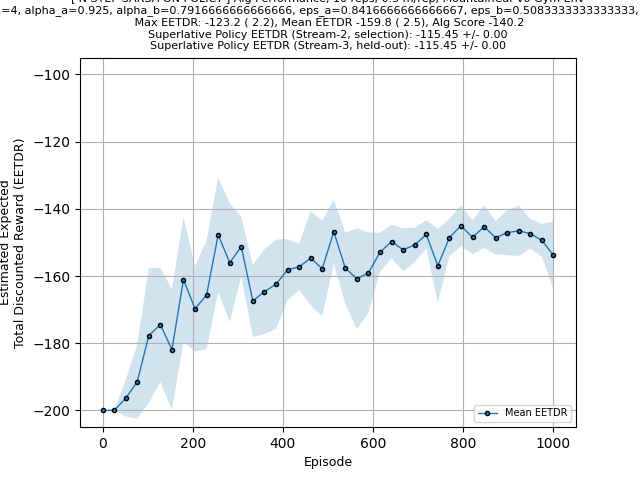
\includegraphics[width=0.7\textwidth]{N_step sarsa LC.png}
    \caption{Learning Curve for Best n-step SARSA run}
\end{figure}
The OLS and ANOVA results are shown below. 
\section*{$n$-step SARSA OLS and ANOVA Regression Results}
\label{sec:nstep_sarsa_statistical_results}

% Unified container for the tables
\begin{table}[htbp]
    \centering
    
    % --- FIRST ROW: OLS SUMMARY & OLS COEFFICIENTS SIDE-BY-SIDE ---
    \begin{subfigure}[b]{0.4\textwidth}
        \centering
        \caption{$n$-step SARSA Model Fit Summary}
        \label{tab:nstep_ols_summary}
        \begin{tabular}{lc}
            \toprule
            \textbf{Metric} & \textbf{Value} \\ 
            \midrule
            $R^2$ & 0.879 \\
            Adj. $R^2$ & 0.776 \\
            $F$-statistic & 8.590 \\
            Prob ($F$-stat) & $2.20 \times 10^{-08}$ \\
            Log-Likelihood & -196.33 \\
            AIC & 448.7 \\
            BIC & 507.3 \\ 
            \bottomrule
        \end{tabular}
    \end{subfigure}
    \hfill
    \begin{subfigure}[b]{0.58\textwidth}
        \centering
        \caption{$n$-step SARSA ANOVA Type II Effects Table}
        \label{tab:nstep_anova_results}
        \begin{tabular}{lrrrc}
            \toprule
            \textbf{Variable} & \textbf{sum\_sq} & \textbf{df} & \textbf{$F$} & \textbf{PR($>F$)} \\ 
            \midrule
            $\alpha_a$ & 71.717430 & 1.0 & 0.939651 & 0.339638 \\
            $\alpha_b$ & 2.149772 & 1.0 & 0.028167 & 0.867774 \\
            $\epsilon_a$ & 84.441042 & 1.0 & 1.106357 & 0.300754 \\
            $\epsilon_b$ & 60.694407 & 1.0 & 0.795226 & 0.379181 \\
            qinit & 55.846242 & 1.0 & 0.731704 & 0.398691 \\
            n\_steps & 288.635678 & 1.0 & 3.781740 & 0.060648 \\ 
            \bottomrule
        \end{tabular}
    \end{subfigure}
    
    
    \vspace{5mm} % Vertical separation between OLS and ANOVA rows
    
    % --- SECOND ROW: ANOVA TABLE ---
   \begin{subfigure}[b]{0.9\textwidth}
        \centering
        \caption{$n$-step SARSA Coefficient Estimates}
        \label{tab:nstep_ols_coefficients}
        \begin{tabular}{lrrrcrc}
            \toprule
            \textbf{Variable} & \textbf{coef} & \textbf{std err} & \textbf{$t$} & \textbf{$P>|t|$} & \multicolumn{2}{c}{\textbf{[0.025 \quad 0.975]}} \\ 
            \midrule
            Intercept & -153.1315 & 15.298 & -10.010 & 0.000 & -184.293 & -121.970 \\
            $\alpha_a$ & -29.3572 & 30.285 & -0.969 & 0.340 & -91.046 & 32.332 \\
            $\alpha_b$ & -4.4412 & 26.463 & -0.168 & 0.868 & -58.344 & 49.461 \\
            $\epsilon_a$ & -27.6490 & 26.286 & -1.052 & 0.301 & -81.193 & 25.895 \\
            $\epsilon_b$ & 22.4809 & 25.210 & 0.892 & 0.379 & -28.870 & 73.832 \\
            qinit & 24.5221 & 28.668 & 0.855 & 0.399 & -33.872 & 82.916 \\
            n\_steps & 49.9917 & 25.707 & 1.945 & 0.061 & -2.372 & 102.355 \\ 
            \bottomrule
        \end{tabular}
    \end{subfigure}

\end{table}
\newpage
From these results the focus shifts from $\epsilon_b$ to n-steps with the highest F-statistic and the lowest p-value. This is due to its power in balancing bias and variance as well as altering the nature of the target the agent is trying to learn. We also see an increase in $R^2$ values compared to the other two methods.

\section{Algorithm Comparison}
\begin{table}[htbp]
\centering
\caption{Executive Summary: Model Fit and Dominant Parameter Effects Across Architectures}
\label{tab:executive_summary_stats}
\resizebox{\textwidth}{!}{%
\begin{tabular}{lcccccccl}
\toprule
 & \multicolumn{4}{c}{\textbf{Overall Model Fit Metrics}} & \multicolumn{4}{c}{\textbf{Primary Driver Performance Impact}} \\ 
\cmidrule(lr){2-5} \cmidrule(lr){6-9}
\textbf{RL Architecture} & \textbf{$R^2$} & \textbf{Adj. $R^2$} & \textbf{$F$-Statistic} & \textbf{Prob ($F$-stat)} & \textbf{Factor} & \textbf{Coefficient} & \textbf{$t$-stat} & \textbf{$P>|t|$} \\ \midrule
On-Policy SARSA & 0.767 & 0.647 & 6.415 & $4.09 \times 10^{-07}$ & $\epsilon_b$ & 80.6979 & 2.844 & 0.007$^{**}$ \\
Off-Policy Q-Learning & 0.786 & 0.676 & 7.168 & $9.38 \times 10^{-08}$ & $\epsilon_b$ & 91.5923 & 3.374 & 0.002$^{**}$ \\
$n$-Step SARSA ($n=6$) & 0.879 & 0.776 & 8.590 & $2.20 \times 10^{-08}$ & \texttt{n\_steps} & 49.9917 & 1.945 & 0.061$^{\dagger}$ \\ \bottomrule
\multicolumn{9}{l}{\small $^{\dagger}$ Significant at the $10\%$ level; $^{*}$ Significant at the $5\%$ level; $^{**}$ Significant at the $1\%$ level.}
\end{tabular}%
}
\end{table}
From the above table we can see that all of the algorithms have a well fit model with high $R^2$ and Adj. $R^2$ values as well as highly significant F-statistics. The dominant driver in the single step methods is $\epsilon_b$ which helps these single step methods better balance exploration and exploitation. Unless told otherwise these methods act greedy or don't with no regard to what has come before. The n-step method however is driven by the number of time steps used in the update which in combination with a good decay rate balancing exploration/exploitation balances the bias and variance in the model. This is ideal for this environment since it is a delayed reward environment where the agent needs to learn from the long term consequences of its actions.
\begin{figure*}[htbp]
    \centering
    
    % === ROW 1: LEFT FIGURE ===
    \begin{subfigure}[b]{0.45\textwidth}
        \centering
        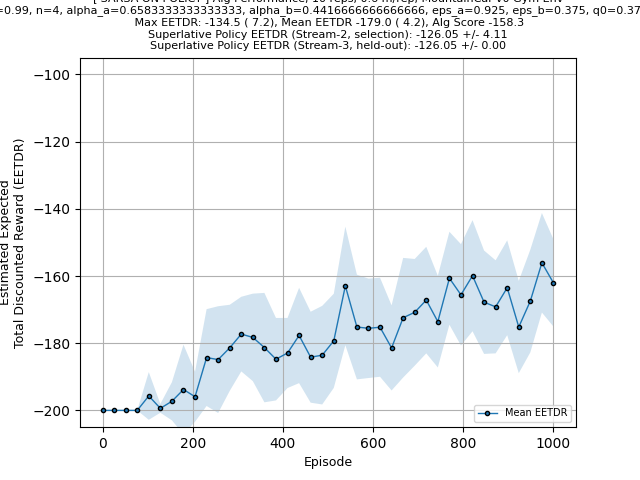
\includegraphics[width=\textwidth]{Q_learning LC.png} 
        \caption{Off-Policy Q-Learning (Run 27.0)}
        \label{fig:sarsa_subplot}
    \end{subfigure}
    \hfill % Pushes the two upper figures to the absolute left and right margins
    % === ROW 1: RIGHT FIGURE ===
    \begin{subfigure}[b]{0.45\textwidth}
        \centering
        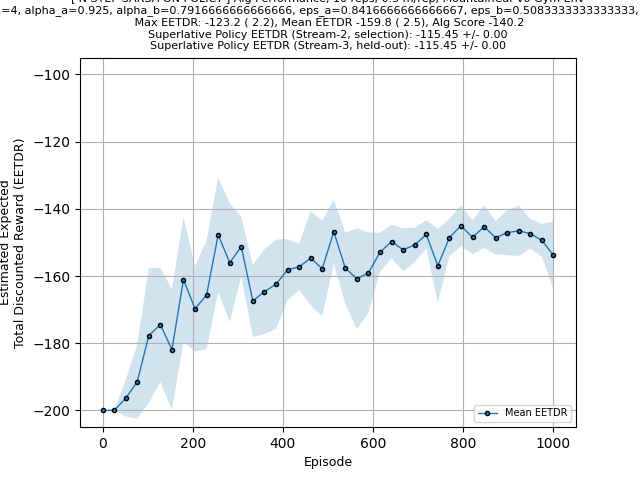
\includegraphics[width=\textwidth]{N_step sarsa LC.png} 
        \caption{Multi-Step $n$-Step SARSA (Run 30.0)}
        \label{fig:q_learning_subplot}
    \end{subfigure}
    
    \vspace{6mm} % Generates vertical breathing room between the two rows   
    % === ROW 2: CENTERED THIRD FIGURE ===
    \begin{subfigure}[b]{0.9\textwidth}
        \centering
        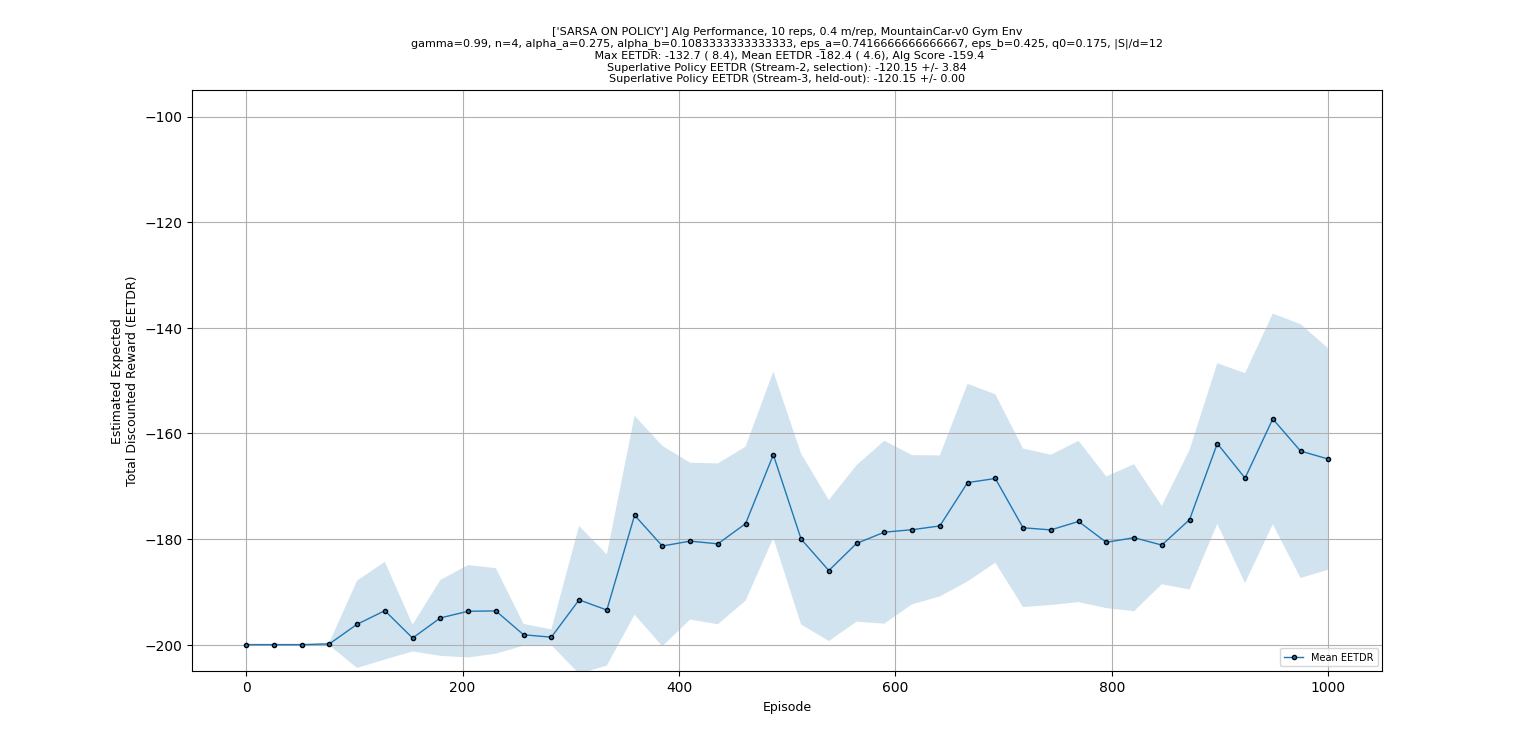
\includegraphics[width=\textwidth]{SARSA LC.png} 
        \caption{On-Policy SARSA (Run 6.0)}
        \label{fig:n_step_sarsa_subplot}
    \end{subfigure}
    
    \caption{Comparative evaluation of learning curves on the MountainCar-v0 environment. The top row contrasts standard 1-step methods, while the bottom row represents the optimized multi-step horizon architecture.}
    \label{fig:rl_comparative_subplots}
\end{figure*}
We see above that the n-step SARSA method has both the tightest variance shading, highest EETDR values, and learns the quickest. Not only that but from previous tables we see the the n-step method is also the fastest to run at 200 seconds per run. For computation time and learning performance the n-step method is the algorithm that is best for this environment. If this were a more reward dense environment the other methods may out perform the n-step method but other tests are needed to confirm this.
\section{Momentum Policy Comparison}
One policy to compare is a fixed policy that is defined as follows:
\begin{align}
    \pi(s) = \begin{cases}
        0 \text{if } s^{velocity}<0\\
        2 \text{otherwise}
    \end{cases}
\end{align}
Statistically speaking this policy ties with both SARSA and Q-learning but is outperformed by the n-step SARSA method. Since it is a fixed policy it also only looks at the immediate situation and state of the car much like the SARSA and Q-learning methods. Again, the agent greatly benefits from having a certain period to learn from and not just the immediate surroundings. The largest difference between the implementations performed above and the momentum policy can be seen in the box and whisker plot below.
\begin{figure}[h]
    \centering
    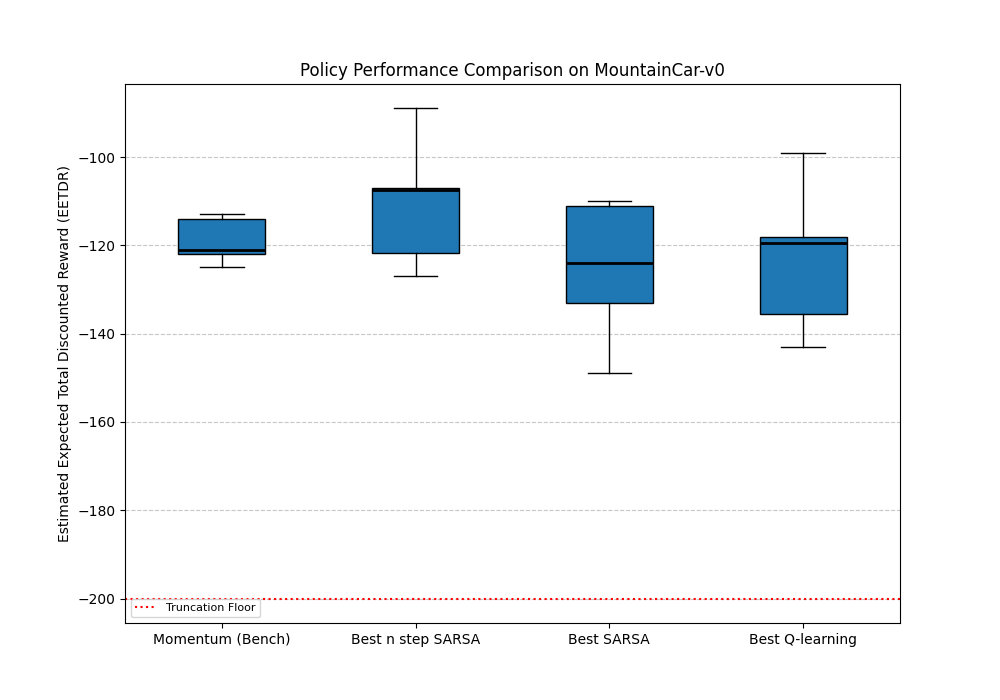
\includegraphics[width=0.8\textwidth]{Policy perfomrance comparison.png}
    \caption{Box and Whisker Plot comparing the EETDR values of the Momentum Policy with the Superlative Policies from each algorithm.}
\end{figure}
\newline
Since the policy is completely fixed it has very little variance as is seen by the tight formation. The policy did not do a terrible job with an average score across the 100 episodes of -119.46 and a 95\% half width of 0.74.
\section{Reflection}
Overall implementing these algorithms to solve the mountain car problem was not extremely difficult due to provided resources. However, ensuring that a balance of hyperparameter tuning design runs and computation time was the largest bottleneck in this project. Each LHD experiment took almost an hour apiece with 60 design runs running in parallel on 10 cores. Since this is a very sparse reward environment and very little to tell the agent how to behave when it is trying to build momentum, novel approaches such as tile coding or the implementation of neural networks may greatly improve the performance since there is more to train in those situations rather than just immediate or short-term rewards. 
\newpage
\section{Appendix: Reinforcement Learning Hyperparameter Design Runs \& Statistical Reports}
\label{sec:appendix_rl_results}

% ==============================================================================
% SECTION 1: SARSA ON-POLICY
% ==============================================================================
\subsection*{1. On-Policy SARSA Experimental Space}

\begin{table*}[htbp]
\centering
\caption{Top 10 Hyperparameter Configurations for On-Policy SARSA (Sorted by Alg Score)}
\label{tab:sarsa_top10}
\resizebox{\textwidth}{!}{%
\begin{tabular}{rccccccccccccc}
\toprule
\textbf{Run Index} & $\alpha_a$ & $\alpha_b$ & $\epsilon_a$ & $\epsilon_b$ & \textbf{qinit} & \textbf{Sup EETDR} & \textbf{Sup EETDR hw} & \textbf{Mean Max EETDR} & \textbf{Mean Max EETDR ME} & \textbf{Time-Avg EETDR} & \textbf{Time-Avg EETDR ME} & \textbf{Secs per run} & \textbf{Alg Score} \\ \midrule
15.0 & 0.241667 & 0.125000 & 0.375000 & 0.358333 & 0.141667 & -124.25 & 6.391664 & -123.84 & 5.793990 & -168.540875 & 4.702179 & 233.409046 & -147.077616 \\
14.0 & 0.591667 & 0.175000 & 0.358333 & 0.275000 & 0.941667 & -114.70 & 7.026125 & -121.72 & 6.493281 & -173.996875 & 4.240568 & 239.248252 & -148.222946 \\
11.0 & 0.558333 & 0.341667 & 0.858333 & 0.308333 & 0.308333 & -120.90 & 6.641154 & -126.61 & 7.049661 & -172.213250 & 3.283964 & 237.255877 & -150.394682 \\
41.0 & 0.991667 & 0.358333 & 0.175000 & 0.325000 & 0.541667 & -125.95 & 6.997147 & -131.36 & 8.751936 & -161.449250 & 4.938806 & 222.037635 & -150.622384 \\
43.0 & 0.825000 & 0.508333 & 0.041667 & 0.758333 & 0.491667 & -130.30 & 13.072783 & -128.26 & 6.269866 & -172.980625 & 4.664217 & 233.549276 & -151.775856 \\
6.0  & 0.275000 & 0.108333 & 0.741667 & 0.425000 & 0.175000 & -127.65 & 5.669851 & -126.75 & 7.230837 & -174.418375 & 4.187460 & 241.776106 & -151.830836 \\
39.0 & 0.841667 & 0.541667 & 0.625000 & 0.908333 & 0.225000 & -115.05 & 6.835465 & -125.83 & 7.910474 & -177.919750 & 4.741719 & 238.083015 & -153.308872 \\
21.0 & 0.341667 & 0.141667 & 0.125000 & 0.825000 & 0.441667 & -127.10 & 6.088733 & -136.03 & 9.456172 & -160.759000 & 4.918814 & 221.155940 & -153.562829 \\
50.0 & 0.091667 & 0.008333 & 0.008333 & 0.341667 & 0.325000 & -127.80 & 5.330998 & -129.96 & 7.607613 & -171.059625 & 8.509056 & 233.948454 & -154.368040 \\
42.0 & 0.441667 & 0.391667 & 0.025000 & 0.441667 & 0.608333 & -115.85 & 7.016561 & -130.89 & 8.335031 & -173.128875 & 4.163171 & 234.302523 & -154.451837 \\ \bottomrule
\end{tabular}%
}
\end{table*}

\begin{table}[htbp]
    \centering
    \begin{subfigure}[b]{0.48\textwidth}
        \centering
        \caption{SARSA Parameter Coefficient Estimates ($R^2 = 0.767$)}
        \label{tab:sarsa_ols}
        \resizebox{\textwidth}{!}{%
        \begin{tabular}{lrrrrrc}
            \toprule
            \textbf{Variable} & \textbf{coef} & \textbf{std err} & \textbf{$t$} & \textbf{$P>|t|$} & \multicolumn{2}{c}{\textbf{[0.025 \quad 0.975]}} \\ \midrule
            Intercept & -189.2700 & 14.027 & -13.494 & 0.000 & -217.642 & -160.899 \\
            $\alpha_a$ & 28.6620 & 33.604 & 0.853 & 0.399 & -39.310 & 96.633 \\
            $\alpha_b$ & -26.5450 & 29.073 & -0.913 & 0.367 & -85.351 & 32.261 \\
            $\epsilon_a$ & 24.7839 & 29.866 & 0.830 & 0.412 & -35.626 & 85.194 \\
            $\epsilon_b$ & 80.6979 & 28.378 & 2.844 & 0.007 & 23.298 & 138.098 \\
            $q_{init}$ & 23.9251 & 32.753 & 0.730 & 0.469 & -42.324 & 90.174 \\
            $\alpha_a^2$ & -11.9534 & 25.464 & -0.469 & 0.641 & -63.460 & 39.553 \\
            $\alpha_a\alpha_b$ & 25.8890 & 20.329 & 1.273 & 0.210 & -15.230 & 67.008 \\
            $\alpha_a\epsilon_a$ & -44.1685 & 22.349 & -1.976 & 0.055 & -89.373 & 1.036 \\
            $\alpha_a\epsilon_b$ & 6.0655 & 18.713 & 0.324 & 0.748 & -31.785 & 43.916 \\
            $\alpha_a q_{init}$ & 7.4305 & 19.602 & 0.379 & 0.707 & -32.219 & 47.080 \\
            $\alpha_b^2$ & -52.6465 & 26.771 & -1.967 & 0.056 & -106.797 & 1.504 \\
            $\alpha_b\epsilon_a$ & 7.4653 & 21.362 & 0.349 & 0.729 & -35.743 & 50.673 \\
            $\alpha_b\epsilon_b$ & -20.0225 & 19.006 & -1.053 & 0.299 & -58.466 & 18.421 \\
            $\alpha_b q_{init}$ & 40.7645 & 20.211 & 2.017 & 0.051 & -0.116 & 81.645 \\
            $\epsilon_a^2$ & -3.4979 & 23.429 & -0.149 & 0.882 & -50.888 & 43.892 \\
            $\epsilon_a\epsilon_b$ & 12.1785 & 21.865 & 0.557 & 0.581 & -32.047 & 56.404 \\
            $\epsilon_a q_{init}$ & -1.1008 & 23.129 & -0.048 & 0.962 & -47.883 & 45.682 \\
            $\epsilon_b^2$ & -59.3983 & 23.446 & -2.533 & 0.015 & -106.822 & -11.975 \\
            $\epsilon_b q_{init}$ & -23.9059 & 18.882 & -1.266 & 0.213 & -62.098 & 14.286 \\
            $q_{init}^2$ & -40.6317 & 21.923 & -1.853 & 0.071 & -84.975 & 3.711 \\ \bottomrule
        \end{tabular}%
        }
    \end{subfigure}
    \hfill
    \begin{subfigure}[b]{0.48\textwidth}
        \centering
        \caption{SARSA ANOVA Type II Breakdown}
        \label{tab:sarsa_anova}
        \resizebox{\textwidth}{!}{%
        \begin{tabular}{lrrrc}
            \toprule
            \textbf{Variable} & \textbf{sum\_sq} & \textbf{df} & \textbf{$F$} & \textbf{PR($>F$)} \\ \midrule
            $\alpha_a$ & 91.614265 & 1.0 & 0.727474 & 0.398911 \\
            $\alpha_b$ & 104.985559 & 1.0 & 0.833650 & 0.366829 \\
            $\epsilon_a$ & 86.721681 & 1.0 & 0.688624 & 0.411684 \\
            $\epsilon_b$ & 1018.372770 & 1.0 & 8.086510 & 0.007065 \\
            $q_{init}$ & 67.197389 & 1.0 & 0.533589 & 0.469468 \\
            $\alpha_a^2$ & 27.749936 & 1.0 & 0.220352 & 0.641386 \\
            $\alpha_a\alpha_b$ & 204.239872 & 1.0 & 1.621791 & 0.210380 \\
            $\alpha_a\epsilon_a$ & 491.891697 & 1.0 & 3.905924 & 0.055219 \\
            $\alpha_a\epsilon_b$ & 13.230765 & 1.0 & 0.105060 & 0.747571 \\
            $\alpha_a q_{init}$ & 18.095788 & 1.0 & 0.143692 & 0.706694 \\
            $\alpha_b^2$ & 487.018217 & 1.0 & 3.867226 & 0.056383 \\
            $\alpha_b\epsilon_a$ & 15.380288 & 1.0 & 0.122129 & 0.728617 \\
            $\alpha_b\epsilon_b$ & 139.762628 & 1.0 & 1.109802 & 0.298608 \\
            $\alpha_b q_{init}$ & 512.310105 & 1.0 & 4.068059 & 0.050623 \\
            $\epsilon_a^2$ & 2.806916 & 1.0 & 0.022289 & 0.882091 \\
            $\epsilon_a\epsilon_b$ & 39.069567 & 1.0 & 0.310237 & 0.580718 \\
            $\epsilon_a q_{init}$ & 0.285276 & 1.0 & 0.002265 & 0.962282 \\
            $\epsilon_b^2$ & 808.292719 & 1.0 & 6.418344 & 0.015426 \\
            $\epsilon_b q_{init}$ & 201.865522 & 1.0 & 1.602937 & 0.212998 \\
            $q_{init}^2$ & 432.594711 & 1.0 & 3.435070 & 0.071402 \\
            Residual & 4911.456033 & 39.0 & \text{NaN} & \text{NaN} \\ \bottomrule
        \end{tabular}%
        }
    \end{subfigure}
\end{table}

\clearpage

% ==============================================================================
% SECTION 2: Q-LEARNING
% ==============================================================================
\subsection*{2. Off-Policy Q-Learning Experimental Space}

\begin{table*}[htbp]
\centering
\caption{Top 10 Hyperparameter Configurations for Off-Policy Q-Learning (Sorted by Alg Score)}
\label{tab:q_top10}
\resizebox{\textwidth}{!}{%
\begin{tabular}{rccccccccccccc}
\toprule
\textbf{Run Index} & $\alpha_a$ & $\alpha_b$ & $\epsilon_a$ & $\epsilon_b$ & \textbf{qinit} & \textbf{Sup EETDR} & \textbf{Sup EETDR hw} & \textbf{Mean Max EETDR} & \textbf{Mean Max EETDR ME} & \textbf{Time-Avg EETDR} & \textbf{Time-Avg EETDR ME} & \textbf{Secs per run} & \textbf{Alg Score} \\ \midrule
43.0 & 0.825000 & 0.508333 & 0.041667 & 0.758333 & 0.491667 & -123.95 & 6.028940 & -126.88 & 5.604704 & -168.781000 & 4.182691 & 250.748533 & -148.676299 \\
15.0 & 0.241667 & 0.125000 & 0.375000 & 0.358333 & 0.141667 & -127.95 & 6.586378 & -123.90 & 4.504471 & -174.078625 & 5.080434 & 263.673305 & -148.706306 \\
14.0 & 0.591667 & 0.175000 & 0.358333 & 0.275000 & 0.941667 & -118.80 & 7.692660 & -124.49 & 6.094680 & -176.659625 & 4.090192 & 269.760487 & -150.650735 \\
53.0 & 0.691667 & 0.525000 & 0.575000 & 0.875000 & 0.458333 & -118.60 & 6.044075 & -126.10 & 6.346384 & -174.840875 & 3.157201 & 258.702947 & -150.667061 \\
11.0 & 0.558333 & 0.341667 & 0.858333 & 0.308333 & 0.308333 & -125.15 & 8.679411 & -127.61 & 8.246403 & -170.753250 & 4.204186 & 262.616913 & -151.496816 \\
41.0 & 0.991667 & 0.358333 & 0.175000 & 0.325000 & 0.541667 & -127.55 & 5.287298 & -137.33 & 4.676498 & -160.762500 & 5.582127 & 242.912153 & -151.741750 \\
27.0 & 0.658333 & 0.441667 & 0.925000 & 0.375000 & 0.375000 & -123.30 & 8.339121 & -132.00 & 6.896231 & -170.493250 & 2.638023 & 258.634193 & -152.590247 \\
36.0 & 0.191667 & 0.241667 & 0.225000 & 0.608333 & 0.191667 & -119.40 & 8.021039 & -130.35 & 7.251462 & -171.768125 & 3.981502 & 256.396496 & -152.860728 \\
42.0 & 0.441667 & 0.391667 & 0.025000 & 0.441667 & 0.608333 & -119.40 & 5.838394 & -130.76 & 7.386290 & -171.793250 & 3.640263 & 252.681322 & -153.061179 \\
32.0 & 0.075000 & 0.041667 & 0.308333 & 0.175000 & 0.475000 & -118.95 & 7.355385 & -129.34 & 6.707078 & -175.987375 & 2.929779 & 266.639413 & -153.195109 \\ \bottomrule
\end{tabular}%
}
\end{table*}

\begin{table}[htbp]
    \centering
    \begin{subfigure}[b]{0.48\textwidth}
        \centering
        \caption{Q-Learning Parameter Coefficient Estimates ($R^2 = 0.786$)}
        \label{tab:q_ols}
        \resizebox{\textwidth}{!}{%
        \begin{tabular}{lrrrrrc}
            \toprule
            \textbf{Variable} & \textbf{coef} & \textbf{std err} & \textbf{$t$} & \textbf{$P>|t|$} & \multicolumn{2}{c}{\textbf{[0.025 \quad 0.975]}} \\ \midrule
            Intercept & -196.5146 & 13.419 & -14.645 & 0.000 & -223.657 & -169.372 \\
            $\alpha_a$ & 44.3574 & 32.149 & 1.380 & 0.176 & -20.669 & 109.384 \\
            $\alpha_b$ & -17.2164 & 27.814 & -0.619 & 0.540 & -73.475 & 39.042 \\
            $\epsilon_a$ & 23.0364 & 28.572 & 0.806 & 0.425 & -34.756 & 80.829 \\
            $\epsilon_b$ & 91.5923 & 27.149 & 3.374 & 0.002 & 36.679 & 146.506 \\
            $q_{init}$ & 30.3175 & 31.334 & 0.968 & 0.339 & -33.062 & 93.697 \\
            $\alpha_a^2$ & -21.5242 & 24.361 & -0.884 & 0.382 & -70.800 & 27.751 \\
            $\alpha_a\alpha_b$ & 27.9053 & 19.448 & 1.435 & 0.159 & -11.433 & 67.243 \\
            $\alpha_a\epsilon_a$ & -44.5845 & 21.380 & -2.085 & 0.044 & -87.831 & -1.339 \\
            $\alpha_a\epsilon_b$ & 2.4875 & 17.902 & 0.139 & 0.890 & -33.723 & 38.698 \\
            $\alpha_a q_{init}$ & -1.2667 & 18.753 & -0.068 & 0.946 & -39.198 & 36.665 \\
            $\alpha_b^2$ & -66.3801 & 25.612 & -2.592 & 0.013 & -118.184 & -14.576 \\
            $\alpha_b\epsilon_a$ & 20.8138 & 20.436 & 1.018 & 0.315 & -20.522 & 62.150 \\
            $\alpha_b\epsilon_b$ & -24.6954 & 18.183 & -1.358 & 0.182 & -61.474 & 12.083 \\
            $\alpha_b q_{init}$ & 42.0229 & 19.335 & 2.173 & 0.036 & 2.913 & 81.132 \\
            $\epsilon_a^2$ & -8.4450 & 22.414 & -0.377 & 0.708 & -53.782 & 36.892 \\
            $\epsilon_a\epsilon_b$ & 8.9894 & 20.918 & 0.430 & 0.670 & -33.320 & 51.299 \\
            $\epsilon_a q_{init}$ & 1.0620 & 22.127 & 0.048 & 0.962 & -43.694 & 45.818 \\
            $\epsilon_b^2$ & -65.6383 & 22.430 & -2.926 & 0.006 & -111.007 & -20.269 \\
            $\epsilon_b q_{init}$ & -20.5097 & 18.064 & -1.135 & 0.263 & -57.047 & 16.028 \\
            $q_{init}^2$ & -45.4899 & 20.973 & -2.169 & 0.036 & -87.912 & -3.068 \\ \bottomrule
        \end{tabular}%
        }
    \end{subfigure}
    \hfill
    \begin{subfigure}[b]{0.48\textwidth}
        \centering
        \caption{Q-Learning ANOVA Type II Breakdown}
        \label{tab:q_anova}
        \resizebox{\textwidth}{!}{%
        \begin{tabular}{lrrrc}
            \toprule
            \textbf{Variable} & \textbf{sum\_sq} & \textbf{df} & \textbf{$F$} & \textbf{PR($>F$)} \\ \midrule
            $\alpha_a$ & 219.424071 & 1.0 & 1.903737 & 0.175520 \\
            $\alpha_b$ & 44.162065 & 1.0 & 0.383153 & 0.539520 \\
            $\epsilon_a$ & 74.923662 & 1.0 & 0.650042 & 0.424987 \\
            $\epsilon_b$ & 1311.898780 & 1.0 & 11.382117 & 0.001687 \\
            $q_{init}$ & 107.901916 & 1.0 & 0.936164 & 0.339229 \\
            $\alpha_a^2$ & 89.977193 & 1.0 & 0.780648 & 0.382357 \\
            $\alpha_a\alpha_b$ & 237.293216 & 1.0 & 2.058771 & 0.159303 \\
            $\alpha_a\epsilon_a$ & 501.202912 & 1.0 & 4.348468 & 0.043635 \\
            $\alpha_a\epsilon_b$ & 2.225252 & 1.0 & 0.019306 & 0.890207 \\
            $\alpha_a q_{init}$ & 0.525871 & 1.0 & 0.004562 & 0.946492 \\
            $\alpha_b^2$ & 774.250879 & 1.0 & 6.717450 & 0.013367 \\
            $\alpha_b\epsilon_a$ & 119.558384 & 1.0 & 1.037296 & 0.314728 \\
            $\alpha_b\epsilon_b$ & 212.610888 & 1.0 & 1.844626 & 0.182215 \\
            $\alpha_b q_{init}$ & 544.427902 & 1.0 & 4.723491 & 0.035889 \\
            $\epsilon_a^2$ & 16.361492 & 1.0 & 0.141953 & 0.708389 \\
            $\epsilon_a\epsilon_b$ & 21.287138 & 1.0 & 0.184689 & 0.669740 \\
            $\epsilon_a q_{init}$ & 0.265540 & 1.0 & 0.002304 & 0.961962 \\
            $\epsilon_b^2$ & 987.042306 & 1.0 & 8.563642 & 0.005694 \\
            $\epsilon_b q_{init}$ & 148.583913 & 1.0 & 1.289123 & 0.263139 \\
            $q_{init}^2$ & 542.226002 & 1.0 & 4.704387 & 0.036245 \\
            Residual & 4495.126115 & 39.0 & \text{NaN} & \text{NaN} \\ \bottomrule
        \end{tabular}%
        }
    \end{subfigure}
\end{table}

\clearpage

% ==============================================================================
% SECTION 3: N-STEP SARSA
% ==============================================================================
\subsection*{3. Multi-Step ($n$-step) SARSA Experimental Space}

\begin{table*}[htbp]
\centering
\caption{Top 10 Hyperparameter Configurations for $n$-step SARSA (Sorted by Alg Score)}
\label{tab:nstep_top10}
\resizebox{\textwidth}{!}{%
\begin{tabular}{rcccccccccccccc}
\toprule
\textbf{Run Index} & $\alpha_a$ & $\alpha_b$ & $\epsilon_a$ & $\epsilon_b$ & \textbf{qinit} & \textbf{n\_steps} & \textbf{Sup EETDR} & \textbf{Sup EETDR hw} & \textbf{Mean Max EETDR} & \textbf{Mean Max EETDR ME} & \textbf{Time-Avg EETDR} & \textbf{Time-Avg EETDR ME} & \textbf{Secs per run} & \textbf{Alg Score} \\ \midrule
11.0 & 0.558333 & 0.341667 & 0.858333 & 0.308333 & 0.308333 & 5.0 & -111.90 & 0.0 & -122.73 & 7.452758 & -145.830625 & 5.648526 & 200.855438 & -127.731660 \\
20.0 & 0.875000 & 0.325000 & 0.141667 & 0.391667 & 0.958333 & 8.0 & -119.55 & 0.0 & -131.06 & 9.295134 & -140.679750 & 9.015519 & 184.464579 & -131.608108 \\
41.0 & 0.991667 & 0.358333 & 0.175000 & 0.325000 & 0.541667 & 3.0 & -118.10 & 0.0 & -130.99 & 8.046902 & -147.120125 & 5.348813 & 187.638711 & -131.847575 \\
27.0 & 0.658333 & 0.441667 & 0.925000 & 0.375000 & 0.375000 & 7.0 & -119.00 & 0.0 & -138.25 & 6.893916 & -146.375375 & 6.673852 & 193.529166 & -132.619691 \\
1.0  & 0.425000 & 0.625000 & 0.458333 & 0.625000 & 0.158333 & 9.0 & -116.35 & 0.0 & -139.03 & 12.528568 & -151.153625 & 7.306442 & 194.182282 & -133.194027 \\
31.0 & 0.625000 & 0.558333 & 0.158333 & 0.658333 & 0.808333 & 3.0 & -117.55 & 0.0 & -121.21 & 3.039561 & -153.134875 & 3.660002 & 193.852888 & -133.247951 \\
15.0 & 0.241667 & 0.125000 & 0.375000 & 0.358333 & 0.141667 & 6.0 & -118.55 & 0.0 & -137.99 & 7.957693 & -150.899875 & 4.874403 & 198.905594 & -133.439711 \\
30.0 & 0.925000 & 0.791667 & 0.841667 & 0.508333 & 0.725000 & 6.0 & -116.95 & 0.0 & -124.29 & 7.357637 & -155.864875 & 3.670496 & 198.145654 & -133.984148 \\
6.0  & 0.275000 & 0.108333 & 0.741667 & 0.425000 & 0.175000 & 4.0 & -116.35 & 0.0 & -129.55 & 6.894186 & -156.351000 & 4.376616 & 202.107249 & -134.101046 \\
36.0 & 0.191667 & 0.241667 & 0.225000 & 0.608333 & 0.191667 & 2.0 & -117.20 & 0.0 & -131.56 & 8.738402 & -153.867750 & 7.268764 & 192.786276 & -134.774605 \\ \bottomrule
\end{tabular}%
}
\end{table*}

\begin{table}[htbp]
    \centering
    \begin{subfigure}[b]{0.48\textwidth}
        \centering
        \caption{$n$-step Parameter Coefficient Estimates ($R^2 = 0.879$)}
        \label{tab:nstep_ols}
        \resizebox{\textwidth}{!}{%
        \begin{tabular}{lrrrrrc}
            \toprule
            \textbf{Variable} & \textbf{coef} & \textbf{std err} & \textbf{$t$} & \textbf{$P>|t|$} & \multicolumn{2}{c}{\textbf{[0.025 \quad 0.975]}} \\ \midrule
            Intercept & -153.1315 & 15.298 & -10.010 & 0.000 & -184.293 & -121.970 \\
            $\alpha_a$ & -29.3572 & 30.285 & -0.969 & 0.340 & -91.046 & 32.332 \\
            $\alpha_b$ & -4.4412 & 26.463 & -0.168 & 0.868 & -58.344 & 49.461 \\
            $\epsilon_a$ & -27.6490 & 26.286 & -1.052 & 0.301 & -81.193 & 25.895 \\
            $\epsilon_b$ & 22.4809 & 25.210 & 0.892 & 0.379 & -28.870 & 73.832 \\
            $q_{init}$ & 24.5221 & 28.668 & 0.855 & 0.399 & -33.872 & 82.916 \\
            n\_steps & 49.9917 & 25.707 & 1.945 & 0.061 & -2.372 & 102.355 \\
            $\alpha_a^2$ & -41.8754 & 22.165 & -1.889 & 0.068 & -87.025 & 3.274 \\
            $\alpha_a\alpha_b$ & 87.8747 & 18.134 & 4.846 & 0.000 & 50.937 & 124.812 \\
            $\alpha_a\epsilon_a$ & -15.1410 & 20.682 & -0.732 & 0.469 & -57.269 & 26.987 \\
            $\alpha_a\epsilon_b$ & 15.6803 & 16.791 & 0.934 & 0.357 & -18.521 & 49.882 \\
            $\alpha_a q_{init}$ & 56.9457 & 19.890 & 2.863 & 0.007 & 16.430 & 97.461 \\
            $\alpha_a$ n\_steps & 26.5185 & 18.294 & 1.450 & 0.157 & -10.746 & 63.783 \\
            $\alpha_b^2$ & -90.4788 & 21.630 & -4.183 & 0.000 & -134.538 & -46.420 \\
            $\alpha_b\epsilon_a$ & 18.1634 & 22.982 & 0.790 & 0.435 & -28.650 & 64.977 \\
            $\alpha_b\epsilon_b$ & 16.1171 & 15.929 & 1.012 & 0.319 & -16.329 & 48.563 \\
            $\alpha_b q_{init}$ & 2.6741 & 17.800 & 0.150 & 0.882 & -33.582 & 38.931 \\
            $\alpha_b$ n\_steps & 26.8467 & 18.463 & 1.454 & 0.156 & -10.762 & 64.455 \\
            $\epsilon_a^2$ & -0.7083 & 22.105 & -0.032 & 0.975 & -45.734 & 44.317 \\
            $\epsilon_a\epsilon_b$ & 57.3320 & 19.319 & 2.968 & 0.006 & 17.980 & 96.684 \\
            $\epsilon_a q_{init}$ & -17.2797 & 21.249 & -0.813 & 0.422 & -60.562 & 26.002 \\
            $\epsilon_a$ n\_steps & 12.8941 & 22.881 & 0.564 & 0.577 & -33.713 & 59.501 \\
            $\epsilon_b^2$ & -70.2489 & 19.765 & -3.554 & 0.001 & -110.509 & -29.989 \\
            $\epsilon_b q_{init}$ & 10.3688 & 15.508 & 0.669 & 0.509 & -21.219 & 41.957 \\
            $\epsilon_b$ n\_steps & -7.7033 & 16.946 & -0.455 & 0.652 & -42.221 & 26.814 \\
            $q_{init}^2$ & -46.9790 & 18.921 & -2.483 & 0.018 & -85.519 & -8.439 \\
            $q_{init}$ n\_steps & -8.8474 & 16.210 & -0.546 & 0.589 & -41.866 & 24.171 \\
            n\_steps$^2$ & -54.3171 & 18.164 & -2.990 & 0.005 & -91.316 & -17.319 \\ \bottomrule
        \end{tabular}%
        }
    \end{subfigure}
    \hfill
    \begin{subfigure}[b]{0.48\textwidth}
        \centering
        \caption{$n$-step ANOVA Type II Breakdown}
        \label{tab:nstep_anova}
        \resizebox{\textwidth}{!}{%
        \begin{tabular}{lrrrc}
            \toprule
            \textbf{Variable} & \textbf{sum\_sq} & \textbf{df} & \textbf{$F$} & \textbf{PR($>F$)} \\ \midrule
            $\alpha_a$ & 71.717430 & 1.0 & 0.939651 & 0.339638 \\
            $\alpha_b$ & 2.149772 & 1.0 & 0.028167 & 0.867774 \\
            $\epsilon_a$ & 84.441042 & 1.0 & 1.106357 & 0.300754 \\
            $\epsilon_b$ & 60.694407 & 1.0 & 0.795226 & 0.379181 \\
            $q_{init}$ & 55.846242 & 1.0 & 0.731704 & 0.398691 \\
            n\_steps & 288.635678 & 1.0 & 3.781740 & 0.060648 \\
            $\alpha_a^2$ & 272.410903 & 1.0 & 3.569161 & 0.067953 \\
            $\alpha_a\alpha_b$ & 1792.303811 & 1.0 & 23.482984 & 0.000031 \\
            $\alpha_a\epsilon_a$ & 40.905487 & 1.0 & 0.535949 & 0.469445 \\
            $\alpha_a\epsilon_b$ & 66.562139 & 1.0 & 0.872105 & 0.357367 \\
            $\alpha_a q_{init}$ & 625.596987 & 1.0 & 8.196648 & 0.007345 \\
            $\alpha_a$ n\_steps & 160.370097 & 1.0 & 2.101189 & 0.156915 \\
            $\alpha_b^2$ & 1335.459918 & 1.0 & 17.497359 & 0.000209 \\
            $\alpha_b\epsilon_a$ & 47.672283 & 1.0 & 0.624608 & 0.435158 \\
            $\alpha_b\epsilon_b$ & 78.139493 & 1.0 & 1.023793 & 0.319211 \\
            $\alpha_b q_{init}$ & 1.722695 & 1.0 & 0.022571 & 0.881521 \\
            $\alpha_b$ n\_steps & 161.370031 & 1.0 & 2.114290 & 0.155668 \\
            $\epsilon_a^2$ & 0.078366 & 1.0 & 0.001027 & 0.974637 \\
            $\epsilon_a\epsilon_b$ & 672.154739 & 1.0 & 8.806654 & 0.005642 \\
            $\epsilon_a q_{init}$ & 50.473985 & 1.0 & 0.661316 & 0.422105 \\
            $\epsilon_a$ n\_steps & 24.237495 & 1.0 & 0.317563 & 0.577004 \\
            $\epsilon_b^2$ & 964.129438 & 1.0 & 12.632142 & 0.001202 \\
            $\epsilon_b q_{init}$ & 34.121275 & 1.0 & 0.447061 & 0.508529 \\
            $\epsilon_b$ n\_steps & 15.771992 & 1.0 & 0.206647 & 0.652477 \\
            $q_{init}^2$ & 470.532258 & 1.0 & 6.164971 & 0.018462 \\
            $q_{init}$ n\_steps & 22.736600 & 1.0 & 0.297898 & 0.588988 \\
            n\_steps$^2$ & 682.520106 & 1.0 & 8.942462 & 0.005324 \\
            Residual & 2442.352384 & 32.0 & \text{NaN} & \text{NaN} \\ \bottomrule
        \end{tabular}%
        }
    \end{subfigure}
\end{table}

\end{document}